\documentclass[14pt]{extarticle}
\usepackage[margin=1in]{geometry}
\usepackage{verbatim}
\usepackage{times}
\usepackage{graphicx}
\usepackage{float}

\begin{document}
\title{Big Data Assignment 2: Hadoop MapReduce Experimentation}
\author{Lee Boyd \\
        Corey Crosser \\
        Sean Soderman
        }
\date{\today}
\maketitle

%TODO: Need graphs in preferably pdf format
\section{Performance graphs}

\begin{figure}[H]
\centering
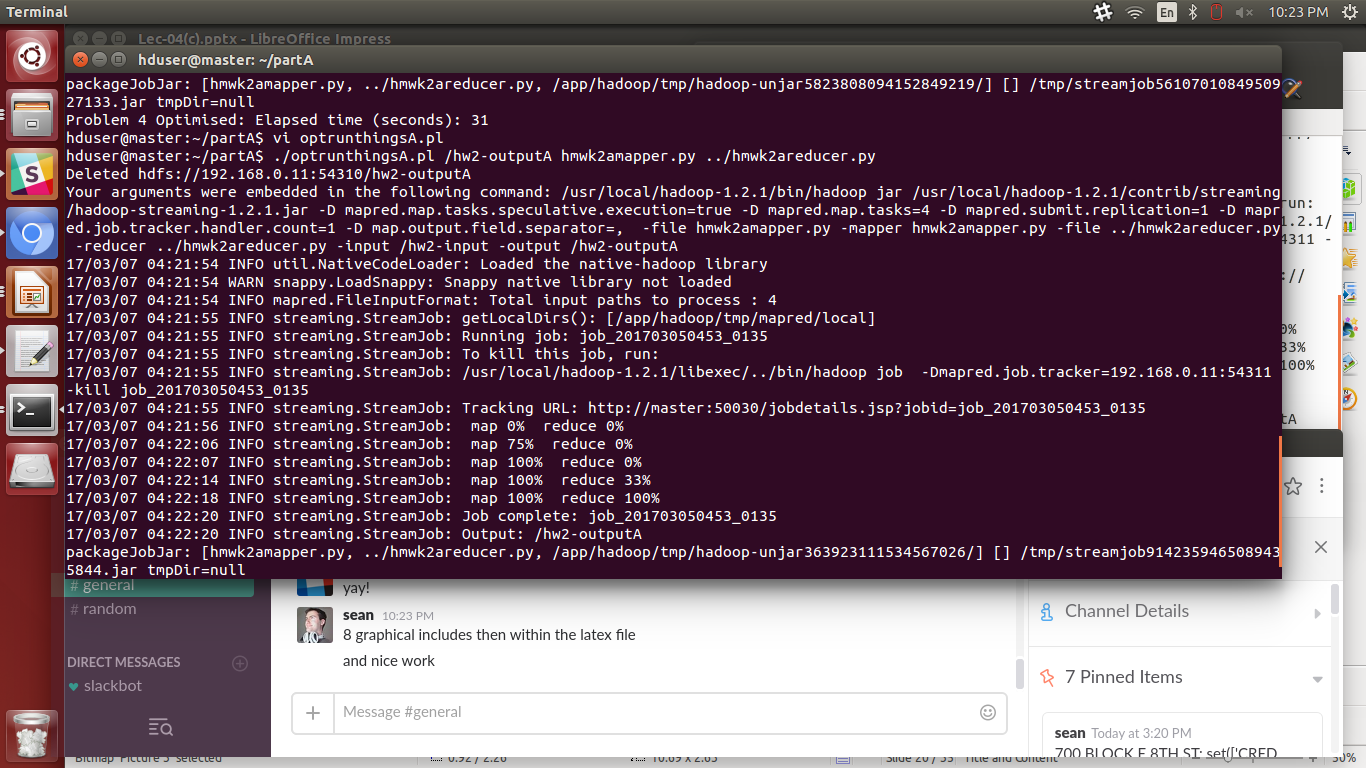
\includegraphics[width=5.2in]{consolescrnshot.png}
\caption{}
\end{figure}

\begin{comment}
\begin{figure}[H]
\centering
\includegraphics[width=5.2in]{}
\caption{}
\end{figure}


\begin{figure}[H]
\centering
\includegraphics[width=5.2in]{}
\caption{}
\end{figure}

\begin{figure}[H]
\centering
\includegraphics[width=5.2in]{}
\caption{}
\end{figure}

\begin{figure}[H]
\centering
\includegraphics[width=5.2in]{}
\caption{}
\end{figure}

\begin{figure}[H]
\centering
\includegraphics[width=5.2in]{}
\caption{}
\end{figure}

\begin{figure}[H]
\centering
\includegraphics[width=5.2in]{}
\caption{}
\end{figure}

\begin{figure}[H]
\centering
\includegraphics[width=5.2in]{}
\caption{}
\end{figure}
\end{comment}


\section{Work Division}
Sean handled the server setup and wrote Perl scripts to ease the formation of relevant MapReduce 
Corey wrote the pseudocode for the mapping and reducing algorithms, including outputs and inputs
Lee translated these algorithms to their Python form and emulated mapreduce for validation and verification. 
We all worked on finding optimization parameters for both parts of the assignment. 

\section{Performance Description}
%TODO
Using the combiner in Part 2 reduced the the shuffle bytes from 32M to 88K, which
would make a significant performance impact in a real network.

\end{document}
